\chapter{Solução proposta: o \ee}
\label{cap:solucao}

O CHOReOS \ee (EE) é um middleware implementado no contexto deste trabalho.
Uma vez instanciado, ele fornece serviços que automatizam
a implantação de composições de serviços\footnote{Como explicado na Seção~\ref{sec:composicoes}, utilizamos os termos 
``composição de serviço'' e ``coreografia'' indistintamente.} 
em ambientes de computação em nuvem,
funcionando no modelo denominado Plataforma como um Serviço (PaaS).
O EE possui funcionalidades e características que foram projetadas para auxiliar o
implantador de composições de grande escala.

Para utilizar o EE, o implantador, usuário do EE, descreve a composição a ser implantada
na Linguagem de Descrição Arquitetural do EE, uma especificação de alto nível que
diz \emph{o que} deve ser implantado, e não o \emph{como}. 
Finalmente, o usuário deve fornecer essa descrição ao EE por meio de sua API remota.

As funcionalidades fornecidas pelo \ee ao usuário são as seguintes:

\begin{itemize}
\item API para automatizar a implantação de composições de serviços em ambientes de computação em nuvem.
\item Criação automatiza de infraestrutura virtualizada (nós na nuvem).
\item Implantação escalável de coreografias de grande escala.
\item Suporte a implantação multi-nuvem.
\item Utilização de serviços de terceiros na composição a ser implantada.
\item Implantação automatizada de infraestrutura de monitoramento dos recursos utilizados.
\item Remoção automática de recursos da nuvem não utilizados.
\item API para escalamento vertical e horizontal.
\end{itemize}

Para a implementação do arcabouço Enactment Engine contribuíram os alunos de pós-graduação Daniel Cuckier, Carlos Eduardo do Santos, Felipe Pontes, Alfonso Diaz, Nelson Lago, Paulo Moura, Thiago Furtado e demais colegas dos projetos Baile e CHOReOS. O \ee é software livre 
sob a Licença Pública Mozilla 2\footnote{\url{http://www.mozilla.org/MPL/2.0/}} 
e está disponível em \url{http://ccsl.ime.usp.br/enactmentengine}. 

Neste capítulo, apresentamos a arquitetura e aspectos de implementação do \ee.   
Destacamos ao final do capítulo
como as decisões arquiteturais e de implementação auxiliam o implantador
a superar os desafios presentes na implantação de composições de grande escala.
Alguns aspectos aqui discutidos são tratados em alto nível,
priorizando o que é importante para o entendimento das contribuições
acadêmicas deste trabalho.
Detalhes técnicos sobre o middleware, principalmente do ponto de vista do
usuário, são encontrados no \userguide (Apêndice~\ref{ape:user_guide}).

\section{Execução do \ee}

O \ee é um sistema de middleware de código aberto que primeiramente deve ser instalado e configurado por um \emph{administrador}.
Uma vez em execução, a instância do EE fornece serviços que podem ser consumidos por algum sistema cliente, desenvolvido
e operado pela figura do \emph{implantador}. O administrador e o implantador podem pertencer à mesma organização,
mas é possível que o administrador forneça o EE como um serviço (SaaS) a terceiros, cobrando por sua utilização.
Para esses terceiros, a vantagem seria evitar o trabalho de instalação e configuração do EE.
O ambiente de execução do EE é exibido na Figura~\ref{fig:arquitetura} e os componentes envolvidos são descritos a seguir.

\begin{figure}[ht]
\centering
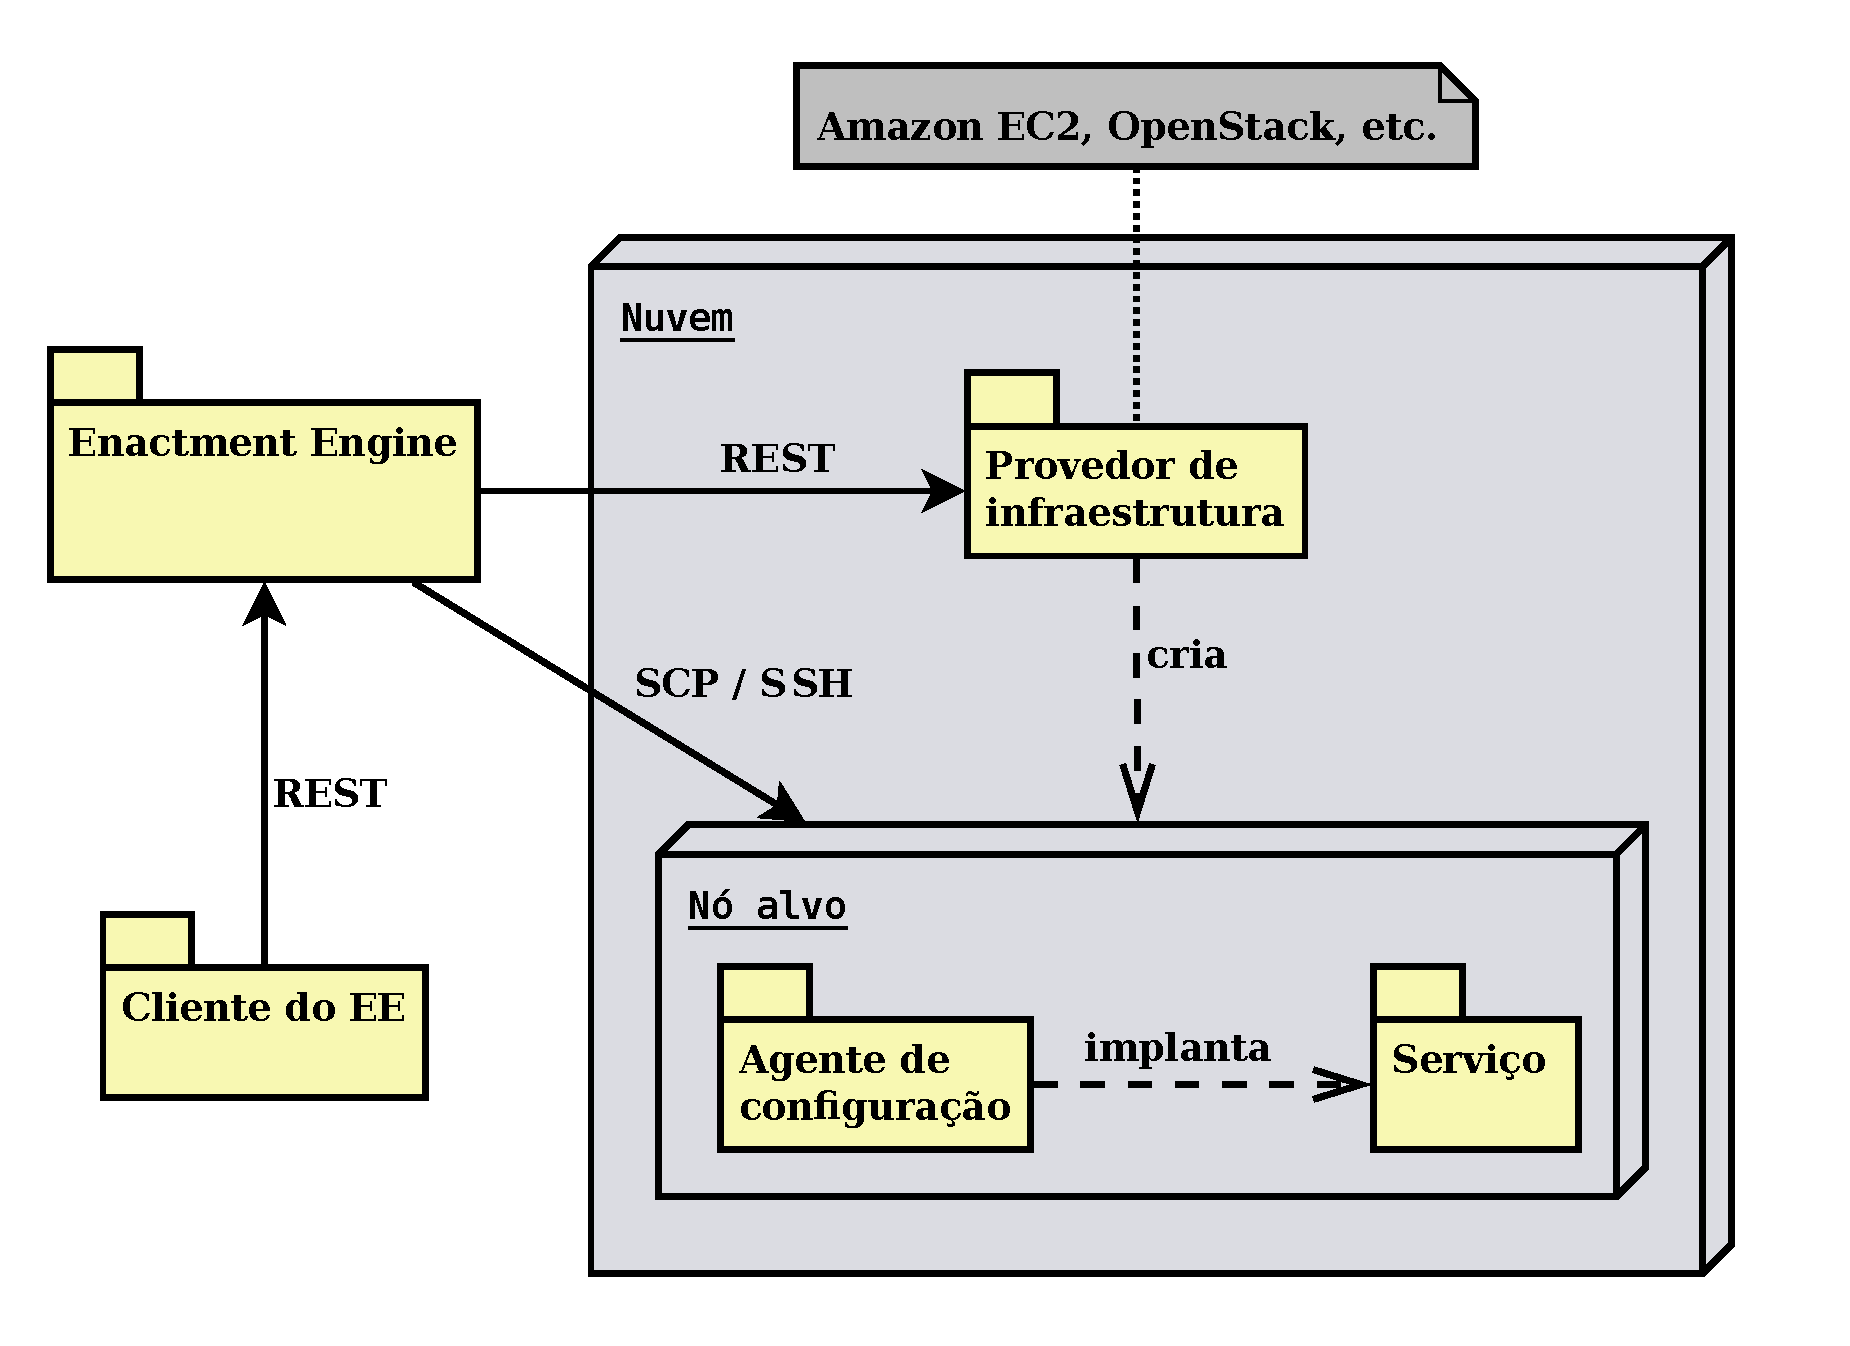
\includegraphics[width=0.7\linewidth]{arquitetura.pdf}
\caption{Ambiente de execução do \choreos \ee.}
\label{fig:arquitetura}
\end{figure}

\begin{itemize}

\item O \emph{provedor de infraestrutura} é um serviço capaz de criar e destruir máquinas virtuais 
(também chamadas de \emph{nós}), normalmente em um ambiente de computação em nuvem. 
Atualmente, o \ee oferece suporte para o Amazon EC2 e o OpenStack.

\item O \emph{agente de configuração} é executado nos nós alvos
e dispara os \scripts que implementam as fases de preparação
e inicialização da implantação dos serviços\footnote{Sobre a nomenclatura das fases de implantação, ver a Seção~\ref{sec:implantacao}.}.
O \ee utiliza o Chef Solo\footnote{\url{http://docs.opscode.com/chef_solo.html}}
como seu agente de configuração.

\item O \emph{cliente do \ee} é um programa ou \script desenvolvido
pelo implantador, no qual a especificação da composição de serviços é definida.
Esse programa deve enviar a especificação da composição para o \ee
por meio das operações REST fornecidas pelo \ee.
Uma opção para implementar essas chamadas é utilizar
a biblioteca Java por nós fornecida, que abstrai os detalhes
das chamadas REST.

\item O \emph{\ee} implanta os serviços de uma composição
com base na especificação enviada pelo cliente.
O processo implementado pelo \ee para efetuar a implantação
é descrito na Figura~\ref{fig:processo}, e explicado logo em seguida. 

\end{itemize} 

A Figura~\ref{fig:processo} exibe o processo de implantação de composições
de serviços implementado pelo \ee:

\begin{figure}[ht]
\centering
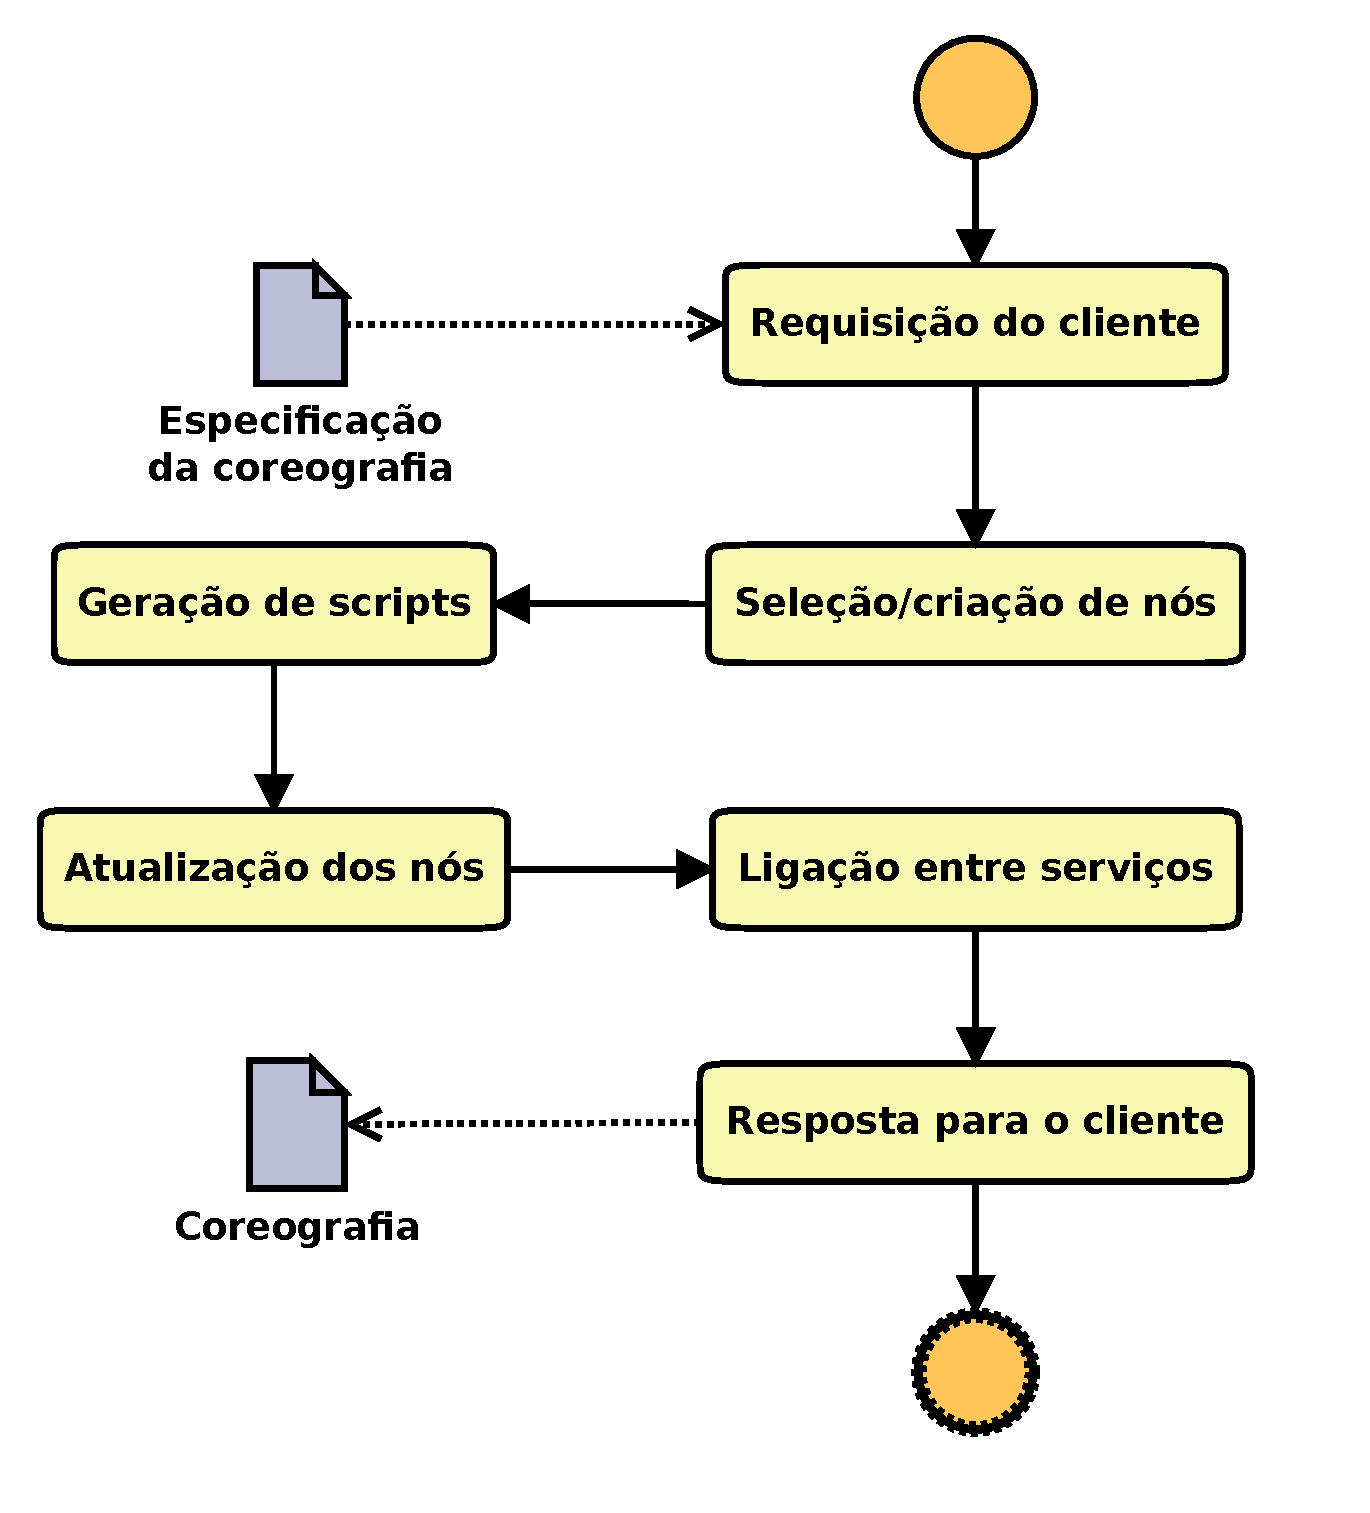
\includegraphics[width=0.5\textwidth]{processo.pdf}
\caption{Processo de implantação implementado pelo \ee.}
\label{fig:processo}
\end{figure}

\begin{enumerate}

\item \emph{Requisição do cliente:} o EE recebe a especificação da composição a ser implantada.
O formato dessa especificação é descrito na Seção~\ref{sec:spec}.

\item \emph{Seleção/criação de nós}: para cada serviço especificado, o EE seleciona um ou mais nós 
onde o serviço será implantado (um serviço pode ter várias réplicas implantadas). 
Se preciso, o EE requisitará ao provedor de infraestrutura a criação de novos nós.
Esse processo de seleção/criação de nós pode levar em conta os requisitos não-funcionais
dos serviços a serem implantados.
A política de seleção de nós é definida pelo administrador do EE, sendo que novas políticas podem ser criadas.

\item \emph{Geração de scripts}: para cada serviço da composição, 
o EE gera dinamicamente os \scripts de preparação do ambiente e inicialização do serviço. 
O EE acessa então o nó alvo selecionado para o serviço,
e configura o agente de configuração desse nó para executar o \script gerado.

\item \emph{Atualização dos nós}: para cada nó alvo que receberá serviços da composição,
o EE dispara a execução do agente de configuração, que por sua vez executa os \scripts 
de preparação e inicialização dos serviços atribuídos ao nó.
Dessa forma, os serviços entram em estado de execução na infraestrutura alvo.

\item \emph{Ligação entre serviços}: após os serviços terem sido iniciados, 
para cada relação de dependência na coreografia (p.ex: serviço \textsf{TravelAgency}
depende do serviço \textsf{Airline}), o EE fornece o endereço da dependência 
(p.ex: \url{http://airline.com/ws}) ao serviço dependente.
Mais informações sobre o processo de ligação são fornecidas na Seção~\ref{sec:ligacao}.

\item \emph{Resposta para o cliente}: o EE responde ao seu cliente,
informando em que nó cada serviço foi implantado
e as URIs de acesso a cada serviço da composição.
O formato da resposta é descrito na Seção~\ref{sec:spec}.

\end{enumerate}

Há também alguns outros passos opcionais que não descrevemos por estarem fora
do escopo deste trabalho. Um exemplo é a implantação da infraestrutura de monitoramento
dos nós alvos. O agente de monitoramento 
(Ganglia\footnote{\url{http://ganglia.sourceforge.net}})
é implantado nos nós alvos pelo EE e
coleta valores de uso de CPU, memória e disco dos nós.

\section{Especificação da composição de serviços}
\label{sec:spec}

O \ee recebe de seus clientes a especificação da composição na forma 
de uma descrição arquitetural com as informações necessárias e suficientes para 
que se possa realizar a implantação da composição. 
O EE também devolve, ao seu cliente, informações sobre o resultado da implantação, 
em especial as localizações de acesso aos serviços. As descrições da composição e de sua 
especificação são feitas por meio de uma \emph{linguagem de descrição arquitetural} (ADL), 
assim como a dos trabalhos vistos no Capítulo~\ref{cap:relacionados}. 
A ADL do EE define a estrutura de classes apresentada na Figura~\ref{fig:adl}. 
Em nossa implementação, representações de instâncias desse modelo 
são trocadas entre o EE e seu cliente em formato XML. 
A descrição detalhada de cada atributo e o esquema XML da linguagem
são apresentados no \userguide.

\begin{figure}[!h]
  \centering
  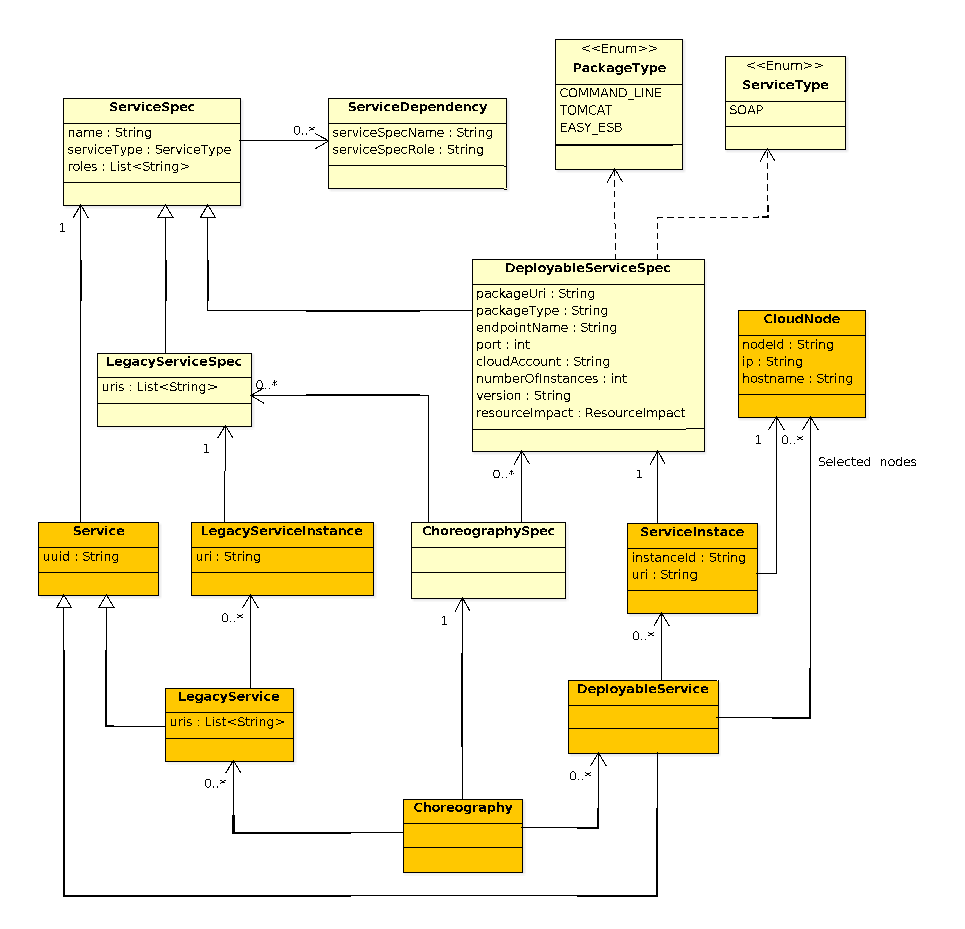
\includegraphics[width=.90\textwidth]{adl.pdf} 
  \caption{Estrutura da descrição arquitetural de uma coreografia.}
  \label{fig:adl} 
\end{figure}

A especificação da coreografia fornece todas as informações para a implantação da composição,
possibilitando que o implantador descreva em alto-nível apenas \emph{o que} deve ser implantado,
e não os detalhes de implementação de \emph{como} deve ser implantado.
Assim, a escrita de uma especificação declarativa se contrapõe à escrita de um \script,
no qual normalmente são descritos os passos de \emph{como} o sistema deve ser implantado.

Na ADL do EE, para cada serviço, especifica-se de onde o pacote do serviço pode ser baixado, 
qual o tipo do pacote (WAR, JAR, etc.), quantas réplicas devem ser implantadas, etc.
Pode-se especificar também a existência de serviços
de terceiros que já estão disponíveis na Internet e que devem
ser consumidos por serviços da composição.

O implantador pode escrever a especificação da coreografia diretamente em XML
ou utilizando objetos Java (POJOs).
A Listagem~\ref{lst:service_spec} apresenta um trecho da especificação escrita em Java,
no qual um dos serviços participantes é definido,
incluindo sua dependência de outro serviço participante.

\lstset{
language=Java,
}

{\scriptsize
\begin{lstlisting}[breaklines, caption={Trecho da especificação de uma coreografia.}, label={lst:service_spec}]
airportBusCompanySpec =
  new DeployableServiceSpec(AIRPORT_BUS_COMPANY, ServiceType.SOAP, PackageType.COMMAND_LINE, resourceImpact, serviceVersion, AIRPORT_BUS_COMPANY_JAR_URL, AIRPORT_BUS_COMPANY_PORT, AIRPORT_BUS_COMPANY, numberOfReplicas);
airportBusCompanySpec.setRoles(
  Collections.singletonList(AIRPORT_BUS_COMPANY));
airportBusCompanySpec.addDependency(
  new ServiceDependency(AIRPORT, AIRPORT_ENDPOINT));
\end{lstlisting}
}

\fabio{listagem acima confusa}

\section{Ligação entre serviços}
\label{sec:ligacao}

Em uma composição de serviços, alguns serviços se comunicam com outros serviços para implementar o fluxo de negócio.
Quando um serviço $A$ invoca um serviço $B$, dizemos que o serviço $A$ depende do serviço $B$. 
Dizemos também que $A$ é \emph{dependente} de $B$, enquanto que $B$ é \emph{dependência} de $A$,
ou ainda que $A$ é \emph{consumidor} de $B$, enquanto $B$ é \emph{provedor} de $A$.
Para que uma coreografia funcione, cada serviço precisa saber o endereço de suas dependências;
o processo pelo qual os serviços recebem os endereços de suas dependências é denominado \emph{ligação}.

\leo{fabio sugere ``enlace dinâmico'' no lugar de ``ligação dinâmica''. Quando aplicar isso, conferir todo o texto.}

Segundo Dearle~\cite{Dearle2007PastPresentFuture}, componentes podem ser ligados entre si em vários momentos: compilação, montagem, configuração e execução. Em nosso contexto, a ligação deve ser efetuada em tempo de execução, pois é somente nesse momento que os endereços completos dos serviços implantados estão disponíveis. Uma das possibilidades apontadas por Dearle para efetivação da ligação em tempo de execução é a utilização do padrão de injeção de dependências, conforme introduzido por Fowler~\cite{Fowler2004Inversion}. A injeção de dependências é utilizada em contêineres como o arcabouço Spring\footnote{\url{http://spring.io}}, no qual o middleware passa ao componente referências de suas dependências. No entanto, Dearle ainda alega que há uma falta de arcabouços para a aplicação da injeção de dependência de forma distribuída.

A solução adotada no \ee para possibilitar a ligação entre serviços envolve a utilização do middleware para a passagem de endereços dos serviços implantados aos seus consumidores. Essa solução consiste na aplicação do padrão de injeção de dependência de forma distribuída, e é similar ao que foi feito nos trabalhos sobre a linguagem Darwin~\cite{Magee1996Dynamic, Magee1994Regis}. 
Note que nessa solução, a ``inteligência'' em determinar quais serviços satisfazem as necessidades de outros serviços está na camada que produz a entrada do EE.
As dependências entre os serviços são definidas na especificação da coreografia,
pela lista de objetos \textsf{ServiceDependency} pertencentes a um \textsf{ServiceSpec}.
Cada serviço na coreografia que possua dependências deve implementar uma operação denominada \texttt{setInvocationAddress}. 
Essa operação, por nós padronizada, recebe como argumentos as seguintes informações sobre a dependência: 

\begin{description}

\item [Papel:] é um nome associado a uma interface, ou seja, define as operações fornecidas por um serviço. A associação entre o nome e 
a interface deve ser previamente acordada pelas organizações participantes da coreografia e a implementação do serviço
deve estar ciente dos nomes e interfaces de suas dependências.

\item [Nome:] é um nome que identifica univocamente o serviço no contexto de uma coreografia. Serve para que o serviço dependente possa 
diferenciar serviços com o mesmo papel. Exemplo: se um serviço de pesquisa de preços utiliza serviços do papel \emph{supermercado},
ele utilizará o nome do serviço para diferenciar os serviços de supermercados diferentes. Com essa semântica, o EE pode atualizar
os endereços de um supermercado com uma nova chamada ao \texttt{setInvocationAddress}, sem que o serviço dependente considere
que se trata de um novo supermercado.

\item [Endereços:] são as URIs das réplicas pelas quais pode-se acessar a dependência.

\end{description}

Assim, em uma coreografia em que, por exemplo, um serviço de agência de viagem dependa do serviço de uma companhia aérea, o EE executa a seguinte invocação ao serviço da agência de viagens : \texttt{setInvocationAddress('Companhia Aérea', 'Nimbus Airline', [ 'http://nimbus.com/ws/' ])}. 

A descrição fornecida até aqui é abstrata e independente de tecnologia.
A definição exata da assinatura da operação deve ser definida de acordo com a tecnologia utilizada.
A versão atual do EE já define essa assinatura para serviços SOAP.
Para detalhes, ver o guia do usuário (Apêndice~\ref{ape:user_guide}).

Apesar dos benefícios da solução adotada no EE, Dearle~\cite{Dearle2007PastPresentFuture} também alerta sobre a desvantagem em forçar componentes a aderirem convenções de codificação impostas pelo middleware, o que poderia restringir o serviço a uma determinada linguagem de programação ou a algum middleware específico. Reconhecemos que esse problema existe em nossa solução, mas acreditamos que o desenho adotado ameniza os problemas levantados, pois tudo o que o serviço é obrigado a fazer é implementar a operação \texttt{setInvocationAddress} e conhecer os papéis de suas dependências, o que implica em conhecer as operações de cada papel. Dessa forma, nossa solução não restringe o serviço a nenhuma linguagem e não impede a utilização do serviço em outro middleware.

\todo{padronizar referências ao guia do usuário, de preferência em pt e referenciando o apêndice}

\section{Mapeamento dos serviços na infraestrutura alvo}
\label{sec:mapeamento}

Em algum momento do processo de implantação, é preciso definir em que nó cada instância de serviço será hospedado.
Chamamos de \emph{mapeamento}, ou seleção de nós, essa fase do processo de implantação.
Na forma mais simples de seleção de nó, o IP do nó alvo é definido estaticamente no \script de implantação do serviço.
O trabalho de Magee e Kramer~\cite{Magee1997Corba} apresenta a seleção de nós em função da utilização de CPUs nos nós existentes, não havendo possibilidade de utilização de outros critérios, como memória, disco, custo etc. Nos sistemas apresentados por Dolstra et al.~\cite{Dolstra2005Configuration} e Balter et al.~\cite{Balter1998Olan} é preciso que a distribuição dos serviços seja especificada com o uso dos IPs das máquinas nas quais os serviços devem ser implantados, o que não é possível em um ambiente de nuvem. Por fim, o \emph{broker} apresentado por Watson et al. é o componente que mais se assemelha ao nosso NodeSelector, pois os autores deixam claro que várias implementações diferentes são possíveis, considerando-se diferentes tipo de requisitos e diferentes fontes de monitoramento. Como a escolha é feita em tempo de execução do serviço, seria também possível uma seleção que independa de IPs estabelecidos em tempo de projeto. No entanto, os autores não explicam como os usuários de seu sistema, os provedores de infraestrutura, deveriam proceder para criar seus próprios \emph{brokers} personalizados.

Para avançar em relação às limitações dos trabalhos anteriormente citados, 
a seleção de nós no \ee
considera os requisitos de dinamicidade do ambiente de nuvem, que nos impede de conhecer os IPs das máquinas 
em tempo de desenvolvimento ou configuração do \script de implantação.
O EE utiliza um seletor de nós automatizado que escolhe em tempo de implantação os nós alvos para um dado serviço.
A escolha de uma política ótima para o seletor é assunto de diversas pesquisas.
Portanto, adotamos aqui uma abordagem extensível, com o fornecimento inicial de políticas como
``sempre cria um novo nó'' ou ``cria nós até um limite, e depois faz rodízio entre eles''.

\section{Interface do \ee}
\label{sec:interface}

Os clientes do \ee utilizam suas funcionalidades por meio de uma API REST, que é descrita nesta seção. 
Por se tratar de uma API REST, o cliente pode ser implementado em qualquer linguagem 
e ambiente que possua alguma biblioteca HTTP. 
Também disponibilizamos um cliente na forma de uma biblioteca na linguagem Java, 
tornando o uso do EE ainda mais simples para os usuários da linguagem Java, 
atualmente uma das mais utilizadas na indústria. 
Seguimos agora com uma descrição de alto nível de cada uma das operações disponíveis 
na API REST do EE. Detalhes da API, como os códigos de estado HTTP devolvidos, 
são fornecidos no guia do usuário (Apêndice~\ref{ape:user_guide}). 
\todo{trocar status HTTP por estado HTTP no resto do texto}

\begin{description}

\item [Criar coreografia:] registra a especificação de uma coreografia no EE. 
Essa especificação é a descrição arquitetural da coreografia, 
estruturada de acordo com a classe \textsf{ChorSpec} (Figura~\ref{fig:adl}). 
Essa operação não realiza a implantação da coreografia.

\item [Obter coreografia:] obtém informações sobre uma coreografia registrada no EE. 
Essas informações referem-se à especificação da coreografia e ao estado da implantação 
de seus serviços, como os nós em que os serviços foram implantados, 
no caso de a implantação já ter sido realizada.

\item [Implantar coreografia:] realiza a implantação de uma coreografia já registrada no EE. 
Ao fim do processo, detalhes do resultado da implantação são retornados de forma estruturada 
de acordo com a classe \textsf{Choreography} (Figura~\ref{fig:adl}).
A implementação dessa operação deve possuir duas importantes propriedades: 
1) a falha na implantação de parte da coreografia não deve interromper a implantação do resto da coreografia; 
2) a operação deve ser \emph{idempotente}, ou seja, uma nova requisição para a implantação da mesma 
coreografia não deve reimplantar os serviços já implantados, 
mas somente aqueles cujas implantações falharam na última execução. 
Para que serviços sejam atualizados, é preciso utilizar um novo valor no atributo ``versão'' da especificação do serviço.

\item [Atualizar coreografia:] registra uma nova versão de uma coreografia no EE. 
Os serviços atualizados na nova versão da coreografia devem possuir 
um novo número de versão em suas especificações. 
Essa operação, assim como a criação da coreografia, não implanta a nova coreografia. 
Para isso, é preciso invocar novamente a operação de implantação.

A atualização de serviços não é o foco de nosso trabalho.
Dessa forma, em nosso trabalho a atualização dos serviços será feita da forma mais simples possível: 
apenas substituindo o serviço existente por sua nova versão. 
Contudo, tal procedimento pode provocar falhas na comunicação entre os serviços de uma coreografia. 
Vários trabalhos \cite{Kramer1990Philosophers, Vandewoude2007Tranquility, Xiaoxing2011VersionConsistent} 
estudam o processo de atualização dinâmica, pelo qual as transações correntes 
são preservadas durante a atualização de um serviço. 
Embora não esteja no escopo de nosso trabalho, esperamos que a arquitetura do EE possa ser 
evoluída para que a operação de atualização de coreografia utilize procedimentos seguros de 
atualização dinâmica, dentre os quais destacamos a proposta de Xiaoxing et al.~\cite{Xiaoxing2011VersionConsistent}.

\end{description}

Na Listagem~\ref{lst:java_chor_enactment}, fornecemos um exemplo de 
um programa Java invocando o EE para implantar uma coreografia.
Nesse exemplo, a classe \textsf{MyChorSpec} encapsula a 
especificação da coreografia.

\begin{lstlisting}[breaklines, caption={Programa Java que invoca o \ee para implantar uma coreografia.}, label={lst:java_chor_enactment}]
public class Deployment {

    public static void main(String[] args) throws DeploymentException, ChoreographyNotFoundException {

        final String EE_URI = "http://myhost:9102/enactmentengine";
        EnactmentEngine ee = new EnactmentEngineClient(EE_URI);
        ChoreographySpec chorSpec = MyChorSpec.getChorSpec();

        String chorId = ee.createChoreography(chorSpec);
        Choreography chor = ee.deployChoreography(chorId);

        System.out.println(chor); // vamos ver o que aconteceu...
    }
}
\end{lstlisting}


\section{Pontos de extensão}
\label{sec:extensao}

Em se tratando de um arcabouço, para lidar com as particularidades do ambiente de cada organização, o Enactment Engine fornece alguns pontos de extensão. Esses pontos de extensão são classes que desenvolvedores devem escrever na linguagem Java e que, de acordo com as configurações do sistema, poderão ser executadas pelo arcabouço.
Neste capítulo descreveremos os pontos de extensão de nosso middleware, 
mostrando as interface associadas a cada um deles.
Para mais detalhes sobre todos os passos necessários para implementar
uma extensão, verificar o guia do usuário (Apêndice~\ref{ape:user_guide}).

\begin{description}

\item [Provedor de infraestrutura:] implementando a interface \textsf{CloudProvider} (Listagem~\ref{lst:cloud_provider}) 
é possível acrescentar ao EE o suporte a novos provedores de infraestrutura. 
Atualmente, o EE oferece suporte para o serviço EC2 do AWS e o OpenStack como provedores de infraestrutura.
Cada um deles possui sua própria implementação de \textsf{CloudProvider}.

\begin{lstlisting}[frame=trbl, label=lst:cloud_provider, caption=Interface CloudProvider.]
public interface CloudProvider {

  public String getCloudProviderName();

  public CloudNode createNode(NodeSpec nodeSpec) throws NodeNotCreatedException;

  public CloudNode getNode(String nodeId) throws NodeNotFoundException;

  public List<CloudNode> getNodes();

  public void destroyNode(String id) throws NodeNotDestroyed, NodeNotFoundException;

  public CloudNode createOrUseExistingNode(NodeSpec nodeSpec) throws NodeNotCreatedException;

  public void setCloudConfiguration(CloudConfiguration cloudConfiguration);

}
\end{lstlisting}

Os métodos da interface \textsf{CloudProvider} referem-se basicamente às operações de CRUD de máquinas virtuais
em uma infraestrutura de nuvem. Além disso, a implementação pode acessar configurações específicas 
através do objeto \texttt{cloudConfiguration}. Tais configurações podem incluir 
credenciais de acesso de uma conta de nuvem (quem paga pelos nós), tipo das instâncias de VMs a serem criadas (afeta preço),
chave de acesso aos nós criados, etc. A Listagem~\ref{lst:cloud_configuration} apresenta um exemplo de configurações
fornecidas à implementação \textsf{AmazonCloudProvider}. 
Essas informações são definida pelo administrador em um arquivo de configuração do EE.

\begin{lstlisting}[frame=trbl, label=lst:cloud_configuration, caption=Configuração do \textsf{AmazonCloudProvider}.]
LEO_AWS_ACCOUNT.CLOUD_PROVIDER=AWS
LEO_AWS_ACCOUNT.AMAZON_ACCESS_KEY_ID=secret!
LEO_AWS_ACCOUNT.AMAZON_SECRET_KEY=secret_too!
LEO_AWS_ACCOUNT.AMAZON_KEY_PAIR=leofl
LEO_AWS_ACCOUNT.AMAZON_PRIVATE_SSH_KEY=/home/leonardo/.ssh/leoflaws.pem
LEO_AWS_ACCOUNT.AMAZON_IMAGE_ID=us-east-1/ami-3337675a
LEO_AWS_ACCOUNT.AMAZON_INSTANCE_TYPE=m1.medium
\end{lstlisting}
 
Para facilitar o desenvolvimento de novas implementações,
nós fornecemos uma implementação base, a classe \textsf{JCloudsCloudProvider}.
Ela utiliza a biblioteca JClouds\footnote{\url{http://jclouds.incubator.apache.org/}},
que já é apta a acessar uma ampla gama de provedores de infraestrutura disponíveis no mercado.
Essa implementação base foi utilizada para a implementação das classes 
\textsf{AmazonCloudProvider} e \textsf{OpenStackKeyStoneCloudProvider},
que contaram, respectivamente, com 79 e 96 linhas de código-fonte.


\item [Política de seleção de nós:] a implementação da interface \textsf{NodeSelector} (Listagem~\ref{lst:node_selector})
define uma nova política de alocação de serviços em nós da nuvem, que pode levar em conta os requisitos não-funcionais do serviço e 
propriedades dos nós à disposição.
Algumas políticas já fornecidas são ``sempre cria um novo nó'' e 
``cria novos nós até um certo limite, depois faz rodízio entre eles''.

\begin{lstlisting}[frame=trbl, label=lst:node_selector, caption=Interface NodeSelector acompanhada de sua classe pai Selector.]
public interface NodeSelector extends Selector<CloudNode, DeployableServiceSpec> {
}

public interface Selector<T, R> {
    public List<T> select(R requirements, int objectsQuantity) throws NotSelectedException;
}
\end{lstlisting}

As implementações de \textsf{NodeSelector} devem criar novos nós ou devolver nós já cadastrados no EE.
Os requisitos não-funcionais podem ser acessados pelo objeto \texttt{deployableServiceSpec} fornecido pelo
middleware à implementação do \textsf{NodeSelector}.
A implementação deve tomar especial cuidado com concorrência, já que o EE mantêm apenas uma instância
por tipo de \textsf{NodeSelector}. Essa característica é importante para que políticas como
rodízio de nós funcionem adequadamente.


\item [Tipos de pacotes de serviços:] um serviço pode ser distribuído por diferentes tipos de pacotes, como em um JAR ou em um WAR, por 
exemplo. Como existem muitas outras opções, é preciso que esse seja um ponto de flexibilidade. Para cada novo tipo de pacote, escreve-se 
um modelo de um \emph{cookbook} Chef que implemente a preparação e a inicialização do serviço. Um \emph{cookbook} possui vários 
arquivos, mas os principais são os arquivos da \emph{receita}, que é o \script de instalação em si, e o arquivo que define \emph
{atributos} a serem usados nas receitas. A Listagem~\ref{lst:recipe_template} mostra a receita do \emph{cookbook} modelo
para implantação de WARs, enquanto que a Listagem~\ref{lst:attributes_template} mostra o arquivo de atributos do mesmo \emph{cookbook}.

\begin{lstlisting}[frame=trbl, label=lst:recipe_template, caption=Receita modelo para a implantação de WARs.]
include_recipe "apt" 
include_recipe "tomcat::choreos"

remote_file "war_file" do
        source "#{node['CHOReOSData']['serviceData']['$NAME']['PackageURL']}"
        path "#{node['tomcat']['webapp_dir']}/$NAME.war"
        mode "0755"
        action :create_if_missing
end

file "#{node['tomcat']['webapp_dir']}/$NAME.war" do
        action :nothing
end
\end{lstlisting}

\begin{lstlisting}[frame=trbl, label=lst:attributes_template, caption=Arquivo modelo de atributos para a implantação de WARs.]
default['CHOReOSData']['serviceData']['$NAME']['PackageURL'] = "$PACKAGE_URL"
\end{lstlisting}

\fabio{e se quiséssemos implantar serviços Ruby ou Python ou C, qual seria a dificuldade e o trabalho necessário?}

Os arquivos listados acima são modelos não executáveis, uma vez que apenas em tempo de implantação 
os símbolos \emph{\$NAME} e \emph{\$PACKAGE\_URL} serão substituídos por valores adequados.
Essa substituição é feita pelo próprio EE.
Ou seja, criar um novo modelo de \emph{cookbok} para o EE significa simplesmente criar um novo \emph{cookbok} Chef
utilizando adequadamente os símbolos \emph{\$NAME} e \emph{\$PACKAGE\_URL}.
O símbolo \emph{\$PACKAGE\_URL} será substituído pela URL do pacote do serviço,
enquanto que o \emph{\$NAME} será substituído por uma identificação única dentro do EE.


\item [Tipos de serviços:] a ligação entre serviços de uma composição depende da passagem de endereços que é feita do \ee para os 
serviços. Para isso, o EE precisa invocar a operação \texttt{setInvocationAddres} dos serviços. A implementação de tal invocação se dá 
de forma diferente de acordo com o tipo de tecnologia de serviço empregada (SOAP ou REST, por exemplo). 
A implementação da interface \textsf{ContextSender} define como a operação \texttt{setInovcationAddress} é invocada. 
Atualmente, o EE possui uma implementação de \textsf{ContextSender}, utilizada para serviços SOAP.
Nota-se que, para cada nova implementação, é preciso definir uma convenção para a assinatura sintática da operação \texttt
{setInvocationAddres}.

\begin{lstlisting}[frame=trbl, label=lst:context_sender, caption=Interface ContextSender.]
public interface ContextSender {
    public void sendContext(String serviceEndpoint, 
                            String partnerRole, 
                            String partnerName, 
                            List<String> partnerEndpoints) throws ContextNotSentException;
}
\end{lstlisting}

\end{description}


\section{Aspectos gerais de implementação}
\label{sec:implementacao}

Nesta seção, descrevemos alguns detalhes sobre a implementação do \ee que 
podem ser especialmente úteis a eventuais desenvolvedores de nosso middleware.
Leitores não interessados nesses aspectos, podem pular diretamente para a Seção~\ref{sec:discussao}.

\begin{description}

\item [Linguagem:] 

O EE é desenvolvido na linguagem Java 6. 
Durante o desenvolvimento utilizamos como ambiente de execução
a JVM OpenJDK 7. O EE é compilado com o Maven 3.

\item [Chef-solo:] 

O Chef é o sistema voltado à implantação de sistemas sobre a qual construímos o \ee.
De certa forma, o EE é uma camada de abstração que facilita o uso do Chef.
A versão utilizada do Chef-Solo é a 11.8.0.
Em versões anteriores do EE, utilizamos o Chef Server,
mas acabamos por abandoná-lo, devido ao gargalo na escalabilidade
que ele gerava, além do pouco benefício funcional que ele agregava.
As receitas Chef são escritas em uma Linguagem Específica de Domínio (DSL) 
que permite a livre
utilização da linguagem Ruby, mas que possui construtos
específicos para as tarefas de implantação, visando proporcionar
principalmente mecanismos de idempotência. Um exemplo pode ser
observado na Listagem~\ref{lst:chef_idempotente}, no qual
se especifica o download de um arquivo que será
baixado somente caso ele ainda não exista no sistema alvo.

\begin{lstlisting}[frame=trbl, label=lst:chef_idempotente, caption=Trecho de receita Chef que ilustra uso de idempotência.]
remote_file "#{node['easyesb']['downloaded_file']}" do
  source "#{node['easyesb']['url']}"
  action :create_if_missing
end
\end{lstlisting}

\item [Apache CXF:]

Uma das principais bibliotecas utilizadas pelo EE é o Apache CXF,
que traz uma série de utilidades para o desenvolvimento de serviços em Java,
dentre elas a implementação do padrão JAX-RS, voltado ao desenvolvimento de serviços REST.

\item [Configuração por imagem:]

Na gerência de configuração de ambientes, há duas abordagens, 
já discutidas na Seção~\ref{sec:cloud}, sobre como configurar um ambiente:
1) utilização de imagem de disco já contendo serviço a ser implantado
e 2) utilização de \scripts para instalação do serviço.
Enquanto a primeira abordagem prima pelo desempenho,
a segunda opção oferece maior flexibilidade e facilidade de evolução.
A abordagem padrão no \ee é se utilizar a configuração por \scripts (gerados pelo EE).
Mas o EE fornece a opção de que o administrador configure qual imagem será
utilizada para criar os nós alvos.
Isso possibilita que o administrador configure uma imagem 
que já contenha o middleware sobre o qual os serviços serão executados.
Assim, se o administrador sabe que o EE será utilizado para implantar WARs,
ele pode configurar uma imagem que já contenha o Tomcat instalado.
Essa abordagem reduz o tempo de implantação.

\item [Testes:] 

Os testes de unidade do \ee são executados com o comando \texttt{mvn test}.
Embora o EE contenha vários testes de unidade e isso seja fundamental,
há uma limitação considerável desses testes, já que executar comandos que
provoquem efeitos colaterais no sistema operacional não é adequado
em testes de unidade. Tais ``efeitos colaterais'' são sempre provocados
durante a execução das receitas Chef.

Por isso, o EE possui também vários testes de \emph{integração} automatizados,
no qual máquinas virtuais são utilizados para a execução de testes nos
quais o EE possa interagir com um sistema operacional.
Esses testes incluem a implantação completa de coreografias.
Embora esses testes sejam importantes para validar o correto funcionamento do sistema,
eles são muito custosos, tanto em termos financeiros quanto de tempo,
uma vez que máquinas virtuais são criadas durante esses testes.

De nossa experiência neste trabalho, acreditamos que
o desenvolvimento de tecnologias de máquinas virtuais
voltadas para o ambiente de teste de aceitação,
de forma que as máquinas sejam criadas mais rapidamente,
seja uma contribuição relevante para a prática de desenvolvimento de software.

\item [Idempotência:] a implementação da operação implantação de forma idempotente considera
que falhas podem acontecer no processo de implantação em cada uma dessas três etapas: 
1) preparação do nó, que consiste na seleção do nó para uma instância, 
incluindo a transferência dos \scripts de implantação para o nó selecionado;
2) a atualização do nó, que é quando os \scripts são executados;
e 3) a ligação entre serviços.

Caso a falha ocorra na \emph{preparação do nó},
o problema poderá ser corrigido na próxima execução da implantação,
pois o EE sempre tenta criar $n_{spec} - n_{instancias}$ instâncias do serviço, 
onde $n_{spec}$ é a quantidade de instâncias que um serviço deve ter
e $n_{instancias}$ é a quantidade de instâncias que um serviço possui no momento.

Para tratar falhas ocorridas na \emph{atualização do nó},
a cada execução da implantação o processo de atualização
é executado em todos os nós novamente.
Nesse passo, o EE está se aproveitando da idempotência dos \scripts
de implantação gerados que, no caso, são receitas Chef.
As receitas utilizam recursos específicos da linguagem do Chef para implementar a idempotência.

Por fim, falhas na \emph{ligação entre serviços} são recuperadas pois todas
as invocações à operação \texttt{setInvocationAddress} são refeitas.
Nesse passo, a idempotência é garantida pela assinatura idempotente
da própria operação \texttt{setInvocationAddress}.

\item [Software livre:] por fim, todas as bibliotecas 
utilizadas pelo \ee são software livre.

\end{description}

\section{Discussão: auxiliando implantações em grande escala}
\label{sec:discussao}

Nesta seção discutimos como as características arquiteturais e de implementação do \ee
impactam na implantação de composições de serviço de grande escala.
Explicamos como o EE contribui para a resolução de cada um dos desafios
apresentados na Seção~\ref{sec:desafios}.
Durante a discussão, destacamos como uma solução de middleware traz vantagens
sobre abordagens \emph{ad-hoc} de implantação em nosso contexto.
Essa discussão, apoiada pelo efetivo funcionamento do EE demonstrado por sua avaliação
(Capítulo~\ref{cap:avaliacao}), fornece também subsídios para a implementação de novos sistemas
de implantação de grande escala, mesmo que não voltados a composições de serviços,
e até mesmo para soluções \emph{ad-hoc}.

\begin{description}

\item [Processo:]

Tornar a implantação de sistemas ``\emph{Internet-scale}'' processos totalmente automatizados
é necessário para que a implantação se torne testável, flexível e confiável~\cite{Hamilton2007InternetScale}
\fabio{frase muito feia. Revisar. E remover esse Internet-Scale em inglês no meio da frase.},
conforme discutido na Seção~\ref{sec:implantacao}.
O EE possibilita a automação do processo de implantação
graças à sua interface remota (REST), que recebe a especificação
da composição a ser implantada e devolve o resultado do processo.
Embora uma interface gráfica para a implantação de composições seja viável,
tal opção não favorece a implantação automatizada,
e, por isso, não foi priorizada em nosso trabalho.

O uso de uma especificação declarativa,
como já utilizado em outros trabalhos~\cite{Balter1998Olan,Magee1996Dynamic},
também facilita o desenvolvimento do \script de implantação
para cada nova composição a ser implantada.
Isso ocorre porque, com uso de uma linguagem declarativa, o implantador descreve em alto nível apenas
\emph{o que} deve ser implantado, e não os detalhes de \emph{como} deve ser implantado.
O uso de linguagens declarativas requer algum tipo de middleware que interprete
a descrição declarativa, executando as ações adequadas.
Portanto, soluções \emph{ad-hoc} dificilmente usariam linguagens declarativas,
sendo em geral orientadas ao uso de \scripts.

O EE segue a tendência atual na implantação de sistemas de grande escala, que é o uso
de recursos elásticos possibilitados pela computação em nuvem.
Recursos virtualizados fornecidos pela nuvem potencializam
a automação do processo de implantação~\cite{Humble2011Continuous}.
Diferentemente dos cenários estudados em trabalhos anteriores sobre
implantação de sistemas baseados em componentes~\cite{Balter1998Olan,Magee1996Dynamic},
em uma infraestrutura de nuvem, os nós alvos são mais dinâmicos. 
Não é possível conhecer os endereços IPs
dos nós alvos quando se está escrevendo a especificação da composição a ser implantada.
A ligação entre serviços é feita em tempo de execução, o que o EE faz via \texttt{setInvocationAddress},
e a política de alocação de nós deve ser flexível, i.e.,
um serviço não deve ser alocado a um IP estático antes do tempo de implantação.
O EE possibilita que políticas de alocação de nós
escolham, em tempo de implantação, em que nós um serviço deve ser implantado,
considerando inclusive o casamento de requisitos não-funcionais do serviço
com características dos nós disponíveis.

\item [Falhas de terceiros:]

Seguindo recomendações gerais feitas por Nygard~\cite{Nygard2009Release},
adotamos no \ee uma abordagem simples para tratar falhas externas.
A lógica de invocação a sistemas externos foi encapsulada em uma classe, 
chamada \textsf{Invoker} (Figura~\ref{fig:invoker}).
Toda vez que se deve acessar um sistema externo, o EE utiliza um \emph{invoker}.
O \textsf{Invoker} recebe os seguintes parâmetros:
uma \emph{tarefa}, que é uma rotina que se comunicará com algum sistema externo,
a quantidade de \emph{tentativas} para executar a tarefa,
o \emph{timeout} de cada tentativa e um \emph{intervalo} entre as tentativas.

Uma instância do \textsf{Invoker} deve ser configurada 
de acordo com sua tarefa (por exemplo, nós descobrimos que três tentativas
não é o suficiente para transferência de arquivos por SCP).
Em vez de ter esses valores fixados no código-fonte, eles são explicitamente
ajustados em arquivos de configuração.
Desta forma, pode-se ajustar esses valores de acordo com 
as características do ambiente alvo.
Portanto, essa abordagem é também uma estratégia para colaborar 
com a heterogeneidade de plataformas e tecnologias.
A classe \textsf{Invoker} pode ser decorada\footnote{Ver padrão de projeto \textsf{Decorator}~\cite{GoF1995Patterns}.} 
para ajustar dinamicamente os valores de timeouts de cada tarefa.
Para implementar essa adaptação, o desenvolvedor tem acesso
ao histórico dos tempos de execução do \emph{invoker}.

\begin{figure}[ht]
\centering
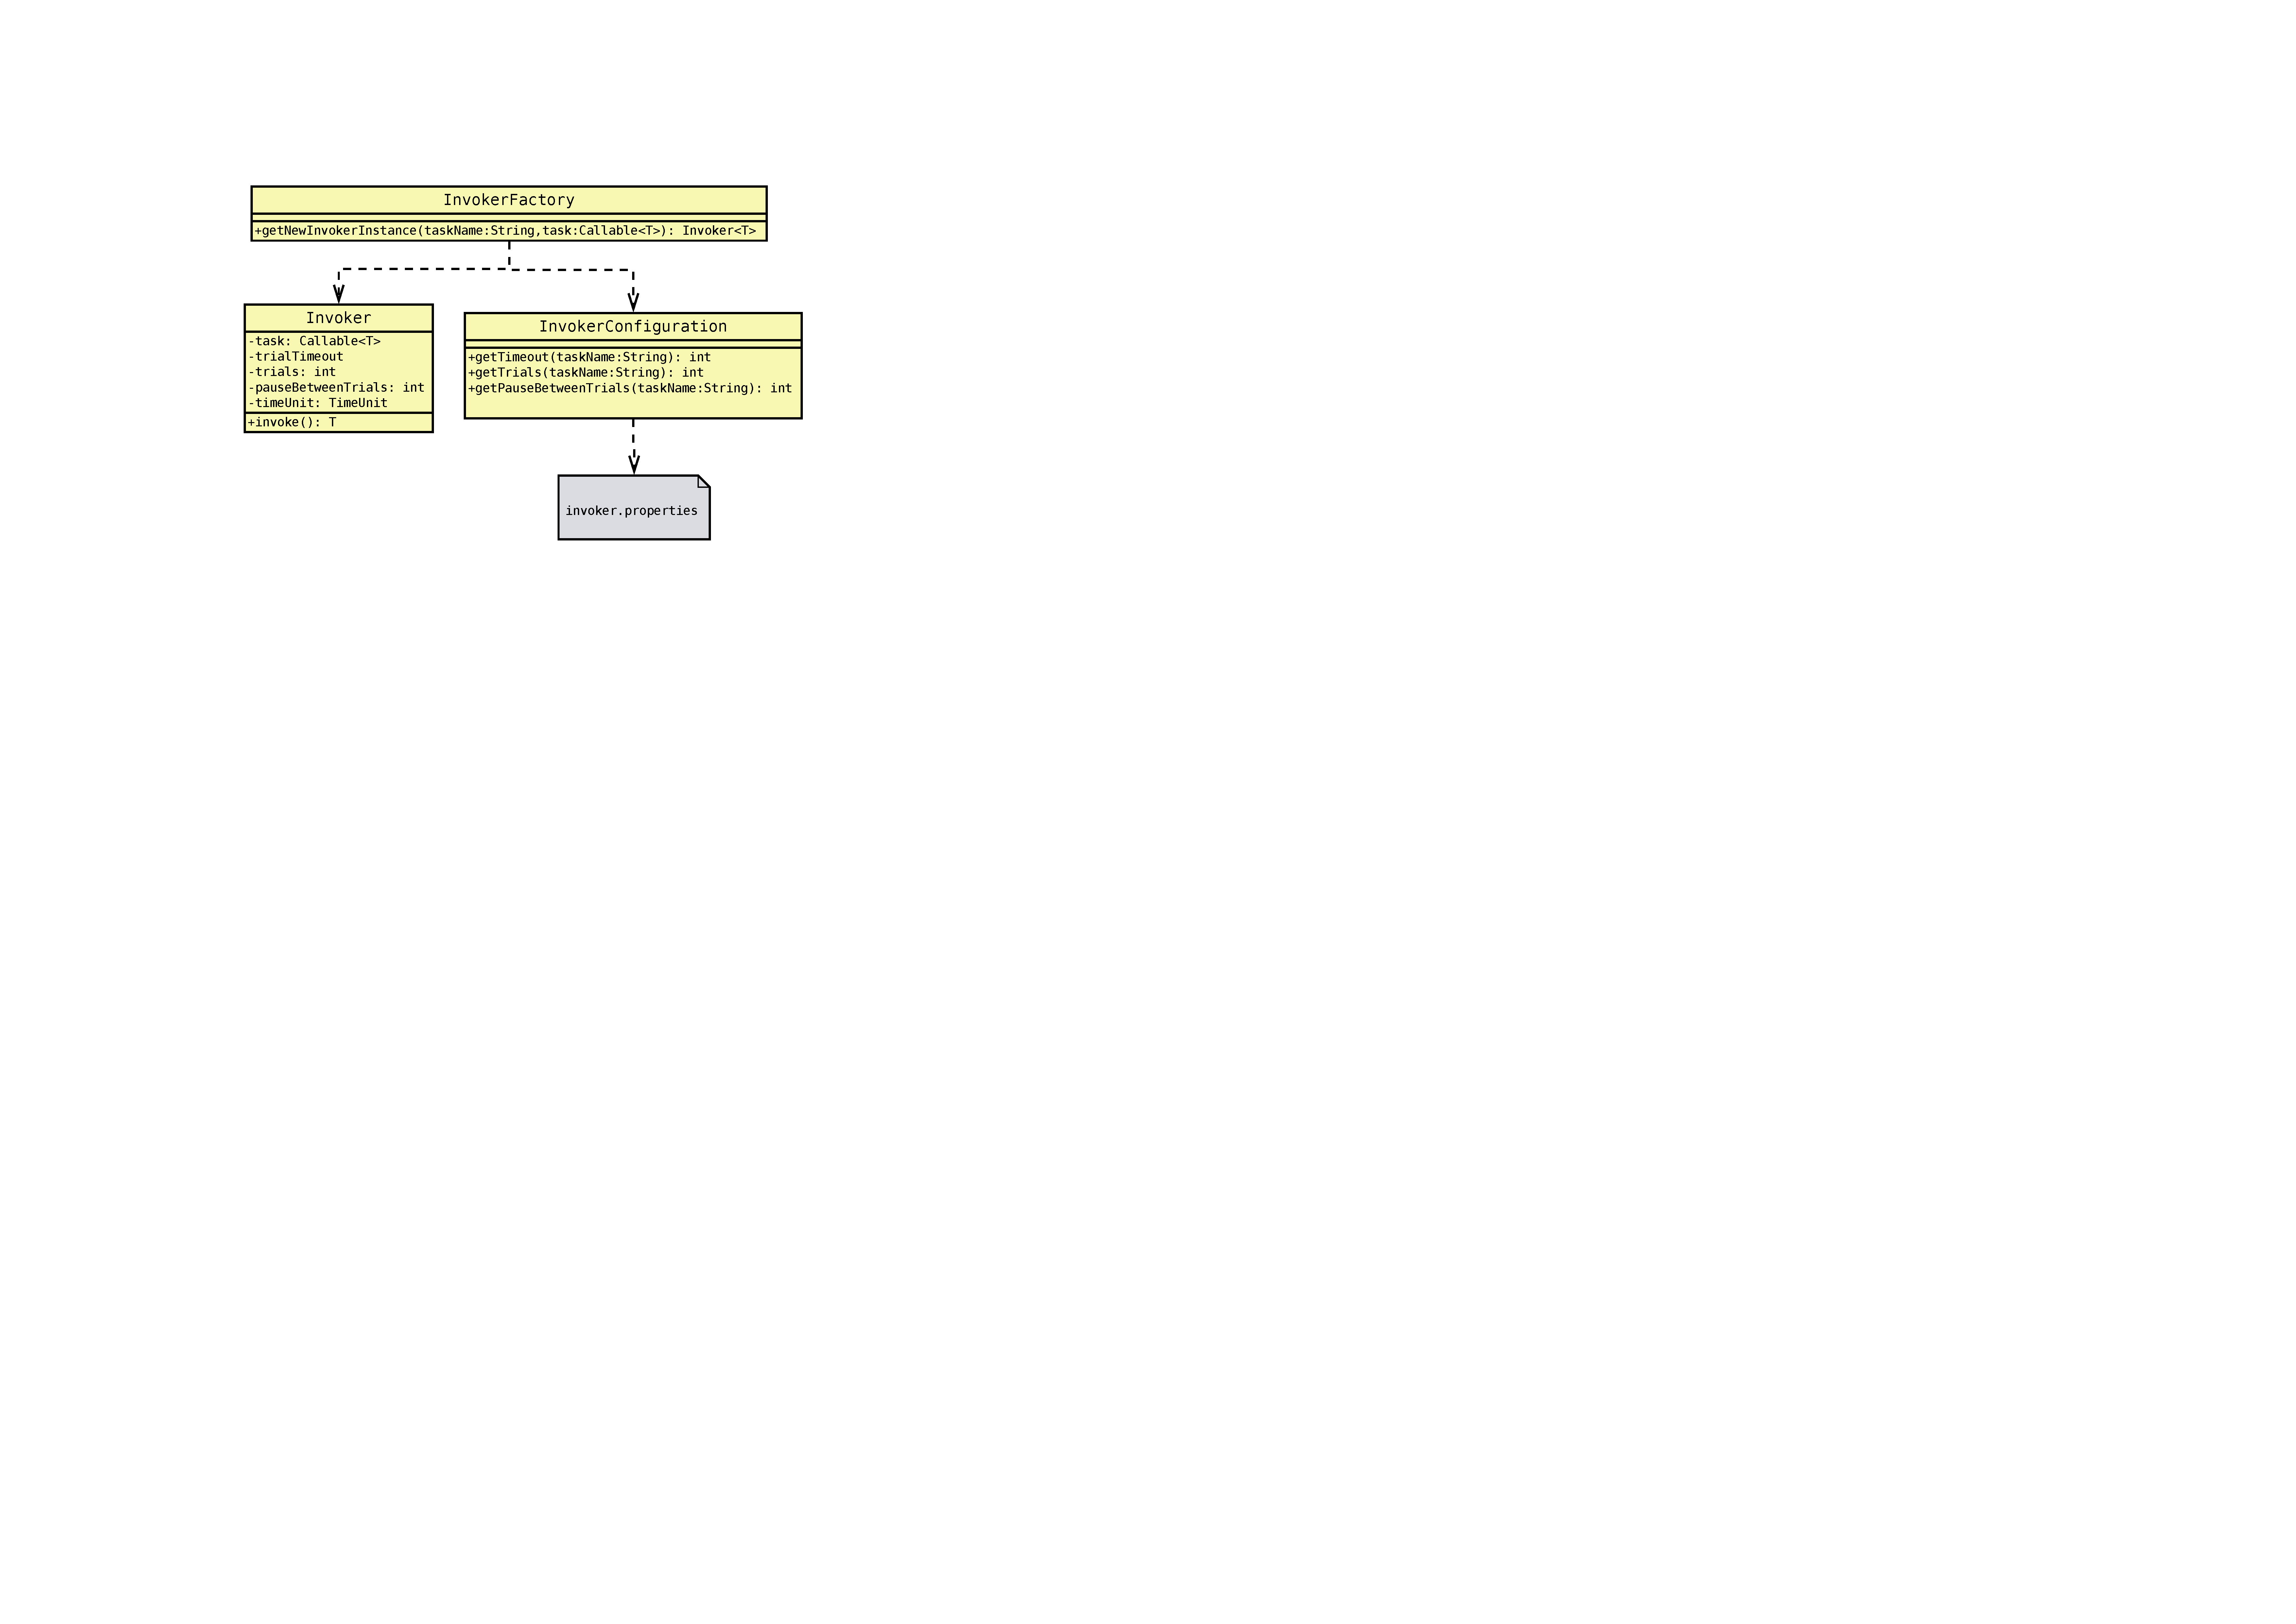
\includegraphics[width=0.6\linewidth]{invoker.pdf}
\caption{Uma instância de \textsf{Invoker} é parametrizada com uma tarefa, uma quantidade de tentativas, um timeout por tentativa e um intervalo de tempo entre as tentativas.}
\label{fig:invoker}
\end{figure}

O EE utiliza os \emph{invokers} nos momentos adequados e necessários.
Isso fornece uma robustez mais facilmente proporcionada por sistemas de middleware,
nos quais interesses transversais podem ser implementados sem que o implantador 
tenha que se preocupar com isso.

\fabio{Esse é o único lugar onde os mecanismos de tolerância a falhas são descritos? 
Essa é uma seção para discussão.  A descrição deveria ter vindo antes.}

O EE adota uma estratégia particular par lidar com falhas durante a criação de novas VMs.
Quando uma requisição chega, o EE tenta criar um novo nó.
Se a criação falha ou demora muito, um nó já criado é recuperado de uma reserva de nós ociosos.
Essa estratégia evita que se tenha que esperar novamente pelo tempo de se criar um novo nó.
A capacidade inicial da reserva é definida por configuração
e ela é preenchida cada vez que a criação de um nó é requisitada.
Se o tamanho da reserva é reduzido e alcança um dado limite,
a capacidade é aumentada, de forma a tentar evitar uma situação futura
de se encontrar uma reserva vazia em um momento de necessidade.

A abordagem da reserva impõe um custo extra de se manter algumas VMs a mais
em execução em um estado ocioso. Contudo, esse problema é tratado
pelo EE por um algoritmo de gerenciamento distribuído em cada nó:
se o nó está em um estado ocioso por $N-1$ minutos, onde $N$ é um limite
de tempo que implica custo adicional, o nó envia ao EE um pedido para 
sua própria finalização. Assim, depois de um tempo de inatividade no EE,
a reserva se torna vazia em algum momento, sendo preenchida novamente
somente quando chegam novas requisições de criação de nós.
%This distributed approach alleviates the need to have the \ee periodically check
%the status of the machines to decide whether they should be removed.

Considerando que o tempo de criação de um nó é bem maior que o tempo de inicialização (\emph{boot})
desse nó, uma melhoria a ser feita na reserva de nós ociosos é manter o nó ocioso desligado
até o momento de uso, uma vez que provedores de infraestrutura, como a Amazon,
costumam não cobrar por máquinas desligadas.
Essa abordagem pode diminuir um pouco o desempenho da reserva de nós,
mas irá economizar mais recursos.

Outra prática importante relacionada a tolerância a falhas é a 
\emph{degradação suave}~\cite{Brewer2001GiantScale,Hamilton2007InternetScale}.
Em nosso contexto, degradação suave significa que se um serviço não foi 
implantado apropriadamente, não é aceitável que o processo de implantação
de toda a composição seja interrompido.
Com o EE, se algum serviço não é implantado, o processo de implantação continua,
e a resposta do EE fornece informações sobre os problemas ocorridos,
possibilitando ações de recuperação.

Contudo, é importante destacar que a responsabilidade pela degradação suave
deve ser compartilhada com a implementação dos serviços, uma vez que cada serviço
deve saber como se comportar na ausência de uma ou mais de suas dependências.
De outra forma, cada serviço se tornaria um \emph{ponto de falha único} na composição,
o que é altamente indesejável.

Por fim, a operação de implantação fornecida pelo EE foi implementada de forma idempotente. 
Isso garante que caso a resposta à requisição 
de implantação de coreografia não chegue ao cliente, o cliente possa repetir a requisição
sem alterar o resultado do processo de implantação. 
Caso a operação de implantação seja chamada pela segunda vez, o EE não implantará
instâncias adicionais de um serviço caso ele já esteja corretamente implantado, mas 
implantará somente as instâncias necessárias para a correta finalização da implantação 
da coreografia. Mais detalhes sobre a implementação da garantia de idempotência, ver a Seção~\ref{sec:implementacao}.

\item [Disponibilidade:]

A especificação de um serviço na ADL do \ee possibilita a definição da quantidade de réplicas
de um serviço a ser implantado pelo EE.
Essa quantidade inicial de réplicas pode ser alterada pelo implantador em tempo de execução
com a atualização da especificação da coreografia.
A definição da quantidade adequada de réplicas, definida pelo implantador, possibilita não só uma melhora
de desempenho, mas também um aumento na disponibilidade do serviço, já que uma falha em uma réplica
específica não afeta as outras réplicas disponíveis.

Por questões de simplificação, em nosso trabalho omitimos a relação que serviços possuem com bancos de dados.
Dessa forma, é importante que versões futuras do EE contemplem a automação da implantação de bancos de dados
a serem utilizados pelos serviços implantados. Nesse estágio, deverá ser considerado também a replicação
do banco de dados, e que os dados são utilizados simultaneamente por várias réplicas do serviço.

\item [Escalabilidade:]

Para implementar o EE, em matéria de programação concorrente, 
não foi preciso saber muito mais que coordenar a abertura e encerramento de múltiplas \emph{threads},
além de sincronizar o acesso a recursos compartilhados por diferentes \emph{threads}.
Assim, depreendemos que o nível de conhecimento de programação concorrente para implementar
um processo de implantação escalável seja básico.
Contudo, programação concorrente por si própria é reconhecida como difícil e propensa a erros. 
Muitas vezes, linguagens de \scripts não oferecem um bom suporte à programação concorrente.
O tratamento adequado de falhas de terceiros também é um requisito importante
para a obtenção de um sistema escalável.
Portanto, implementar concorrência e tratamento a falhas na camada de middlware
é um passo significativo para facilitar a implementação efetiva de um
processo de implantação escalável.

Uma lição aprendida na prática para se atingir a escalabilidade
foi evitar componentes que se tornem gargalos no sistema.
Em versões anteriores do EE, o Chef Server era um ponto central
constantemente requisitado por processos em outros nós.
A mudança da arquitetura do EE da utilização do Chef Server
para o Chef Solo\footnote{Na versão Chef Solo, o EE passa os \scripts de implantação
diretamente ao nó onde o \script será executado. Já com o Chef Server, esses \scripts eram
primeiro armazenados no Chef Server, para depois serem acessados 
pelos nós envolvidos na implantação.} 
foi essencial para se obter desempenhos razoáveis
com uma grande quantidade de serviços implantados..

No Capítulo~\ref{cap:avaliacao}, apresentamos a avaliação em detalhes da 
escalabilidade fornecida pelo \ee.

\item [Heterogeneidade:]

Na Seção~\ref{sec:extensao}, apresentamos os pontos de extensão do \ee,
que possibilitam mais facilmente adaptá-lo para diversos provedores de infraestrutura
e tecnologias de desenvolvimento e empacotamento de serviços.
Essa flexibilidade ajuda a superar
as atuais limitações de soluções de Plataformas como um Serviço
que restrigem as opções tecnológicas disponíveis aos desenvolvedores de aplicações.
Essas restrições normalmente se aplicam justamente sobre
provedor de infraestruturas e a linguagem de programação da aplicação.
Exemplos: para utilizar o PaaS da Amazon (Elastic Beanstalk) é preciso utilizar
o IaaS da Amazon, enquanto que para utilizar o PaaS do Google (App Engine)
é preciso escolher entre as linguagens Java, Pyhton, PHP ou Go.

Oferecer suporte a variações de um padrão é um desafio para sistemas de middleware.
Adequar um middleware para a particularidade de uma aplicação pode não ser fácil.
No suporte a diferentes tecnologias, as abordagens \emph{ad-hoc} encontram realmente um espaço de importância.
No entanto, uma vez que a adequação para uma nova tecnologia seja feita no middleware,
o esforço para o desenvolvimento de futuras aplicações utilizando a mesma tecnologia
se torna menor.

\item [Múltiplas organizações:]

O \ee possui dois principais mecanismos para implantar composições cujos serviços
pertencem a diferentes organizações.
O primeiro mecanismo é a definição da ``conta de nuvem'' a ser usada na implantação de um serviço.
Essa definição é feita na especificação do serviço e deve bater com configurações
previamente feitas pelo administrador no EE.
Uma ``conta de nuvem'' não indica apenas a nuvem alvo (Amazon, por exemplo),
mas também quem vai pagar pela infraestrutura (qual conta da Amazon será utilizada, por exemplo).
Uma vez que os serviços de cada organização sejam configurados para serem implantados
nas contas de nuvem adequadas, o EE irá implantar adequadamente uma composição
multi-organizacional.
No entanto essa abordagem ainda apresenta limitações sérias no quesito de segurança,
pois a configuração da conta de nuvem deve ser fornecida ao administrador do EE,
que seria uma das organizações ou um terceiro.
Esse e outros problemas surgem do fato que diferentes organizações teriam que
compartilhar uma mesma instância do EE.

O segundo mecanismo é a utilização da entidade \emph{serviço legado} na especificação da composição.
O serviço legado é um serviço já existente na Internet, e que portanto
não será implantado pelo EE.
A utilidade de utilizar esse mecanismo está na fase de ligação
entre serviços, pois o EE irá fornecer
aos serviços implantados os endereços dos serviços legados declarados como suas dependências.
A maior limitação dessa abordagem é a dificuldade em se lidar com a alteração de URIs
dos serviços legados.
Quando isso ocorre, uma nova especificação da composição deve ser feita e enviada ao EE,
mas o problema é saber \emph{quando} isso deve ser feito.

Considerando as limitações dos mecanismos até aqui implementados,
divisamos como importante trabalho futuro uma arquitetura de federação entre instâncias do EE.
Caso um serviço $S_A$, implantado com o EE pela organização $O_A$, dependa de um serviço legado $B$,
também implantado com o EE, mas para a organização $O_B$, a instância do EE em $O_B$ poderia
manter a instância do EE em $O_A$ informada sobre o estado de $S_B$.
Para que essa funcionalidade seja implementada é preciso projetar um protocolo
de comunicação entre instâncias do EE.

Nesse estágio proposto (federação dos sistemas implantadores de cada organização) uma abordagem
orientada a middleware se torna importante por questão de padronização.
Abordagens \emph{ad-hoc} deveriam ser desenvolvidas de forma coordenada entre as diferentes organizações,
o que seria mais custoso do que a adoção de uma plataforma comum.

\item [Adaptabilidade:]

O \ee por si só não garante que uma composição será autônoma ou auto-adaptativa.
Contudo, ele fornece suporte para o desenvolvimento de tais sistemas.

Sistemas auto-adaptativos e autonômicos precisam estar cientes
e ter pleno controle das atividades de implantação.
Para equipar tais sistemas, o EE fornece informação e controle
das seguintes funcionalidades:

\begin{itemize}
\item atualização das composições;
\item migração de serviços;
\item replicação de serviços;
\item implantação de infraestrutura de monitoramento.
\end{itemize}

Atualizações de composições de serviços podem ser necessárias quando
as regras de negócio ou os requisitos não-funcionais mudam.
O EE possibilita, por uma API REST, a adição, remoção e reconfiguração dos serviços
e seus recursos computacionais associados.

A migração de um serviço para um nó com mais recursos computacionais
é uma funcionalidade oferecida pelo EE chamada de \emph{escalamento vertical}~\cite{Pritchett2008Base}.
No entanto, para a construção de sistemas escaláveis se recomenda 
a replicação de serviços associada ao balanceamento de carga~\cite{Amazon2012Practices},
o que é conhecido como \emph{escalamento horizontal}~\cite{Pritchett2008Base}.

O EE possibilita a replicação de serviço por meio da implantação de
múltiplas instâncias do serviço e da notificação aos serviços consumidores
sobre a existência dessas réplicas durante a fase de ligação de serviços.
A quantidade inicial de réplicas é definida por atributo na especificação
do serviço fornecida ao EE, e, depois, pode ser redefinida dinamicamente.
Um trabalho futuro é configurar automaticamente um balanceamento de carga
entre réplicas de um serviço, de forma que o consumidor de um serviço
não tenha necessidade de saber sobre suas diversas réplicas.

Por fim, o EE fornece opcionalmente a implantação de uma infraestrutura de monitoramento na infraestrutura alvo.
Utilizamos o Ganglia, que coleta métricas do sistema operacional, como consumo de CPU, por exemplo.
As métricas coletadas são enviadas a um serviço previamente configurado no EE.
Esse serviço de monitoramento pode então disparar ações de adaptação com base
nos dados recebidos. Uma ação de adaptação envolve a geração de uma nova especificação
de composição e a atualização da composição em execução de acordo com a nova especificação.

O CHOReOS \ee é uma ferramenta útil a profissionais da indústria e pesquisadores para
a implantação de composições de serviços, especialmente no contexto de grande escala.
Mas as funcionalidades relacionadas à adaptação são de especial interesse
aos pesquisadores que trabalham com a auto-adaptação de composições de serviços.
O EE facilita a implementação de sistemas adaptativos
por possibilitar que pesquisadores se foquem mais nos problemas de adaptação em
alto nível, abstraindo detalhes altamente específicos do gerenciamento de implantação.
Diferentes pesquisadores desse campo de pesquisa podem se beneficiar ao utilizarem uma plataforma comum,
potencializando a troca de experiência sobre o processo de implantação. 

\end{description}

